%       \\\ ///      %
%       ( @ @ )      %
% ---o00o.(_).o00o---%
%  Maximilian Bandle %
%  bandle@in.tum.de  %
%  Thesis Template   %
% -------------------%
% \documentclass[draft,headsepline,footsepline,footinclude=false,fontsize=11pt,paper=a4,listof=totoc,bibliography=totoc,BCOR=12mm,DIV=15]{scrbook} % two-sided
\documentclass[headsepline,footsepline,footinclude=false,oneside,fontsize=11pt,paper=a4,listof=totoc,bibliography=totoc]{scrbook} % one-sided

\newcommand*{\getUniversity}{Technische Universität München}
\newcommand*{\getFaculty}{School of Computation, Information and Technology --- Informatics}
% Insert your title here
\newcommand*{\getTitle}{Effects of Linux VFIO for User Space I/O}
\newcommand*{\getTitleGer}{Effekt von Linux VFIO auf User Space E/A}
% Insert your name here
\newcommand*{\getAuthor}{Adrian Simon Würth}
% Type of the document
\newcommand*{\getDoctype}{Bachelor's Thesis in Informatics}
% Choose your supervisor
%\newcommand*{\getSupervisor}{Prof. Alfons Kemper, Ph.D.}
\newcommand*{\getSupervisor}{Prof. Dr. Thomas Neumann}
% \newcommand*{\getSupervisor}{Prof. Dr. Jana Giceva}
% Insert your Advisor
\newcommand*{\getAdvisor}{Simon Ellmann, M.Sc.}
% Official submission date
\newcommand*{\getSubmissionDate}{August 15, 2024}
\newcommand*{\getSubmissionLocation}{Munich}

\PassOptionsToPackage{table,svgnames,dvipsnames}{xcolor}

\usepackage[utf8]{inputenc}
\usepackage[T1]{fontenc}
\usepackage[sc]{mathpazo}
\usepackage[american]{babel}
\usepackage[autostyle]{csquotes}
\usepackage[%
  % backend=biber, % somehow biber did not work properly with latexrun. If you find a solution, feel free to open a merge request
  backend=bibtex,
  url=false,
  style=alphabetic,
  maxnames=4,
  minnames=3,
  maxbibnames=99,
  giveninits,
  uniquename=init]{biblatex}
\usepackage[final]{graphicx}
\usepackage{xcolor}
\usepackage{textcomp}
\usepackage{scrhack} % necessary for listings package
\usepackage[final]{listings}
\usepackage{lstautogobble}
\usepackage{tikz}
\usepackage{booktabs}
\usepackage[labelfont=bf]{caption}
\usepackage[final]{microtype}
\usepackage[final, hidelinks, pdfusetitle]{hyperref} % hidelinks removes colored boxes around references and links
\usepackage{multirow}

\usepackage{setspace}
\usepackage{subcaption}

\hypersetup{
  pdftitle={\getTitle},
  pdfsubject={\getDoctype},
  pdfauthor={\getAuthor},
  pdfkeywords={}
}

\usepackage{float}
\usepackage{algorithm}
\usepackage[noend]{algpseudocode}

\newcommand{\imagePath}[1]{figures/#1}

\bibliography{bibliography}

\setkomafont{disposition}{\normalfont\bfseries} % use serif font for headings
\linespread{1.05} % adjust line spread for mathpazo font

% TUM Colors
\definecolor{TUMblue}{RGB}{0,101,189} % TUMBlau

% 150 Years
\definecolor{TUMgreen}{RGB}{161,191,22} % Gruen
\definecolor{TUMpink}{RGB}{227,130,143} % Rosa
\definecolor{TUMorange}{RGB}{243,145,0} % Orange
\definecolor{TUMbrown}{RGB}{202,171,41} % Senf
\definecolor{TUMblueLight}{RGB}{91,197,242}  % Hellblau

% 150 Years (Light)
\definecolor{TUMlightGreen}{RGB}{188,207,30} % Gruen
\definecolor{TUMlightPink}{RGB}{242,144,149} % Rosa
\definecolor{TUMlightOrange}{RGB}{247,166,0} % Orange
\definecolor{TUMlightBrown}{RGB}{232,200,55} % Senf
\definecolor{TUMlightBlueLight}{RGB}{146,212,241} % Hellblau

% Settings for algorithm
\algnewcommand\algorithmicforeach{\textbf{for each}}
\algdef{S}[FOR]{ForEach}[1]{\algorithmicforeach\ #1\ \algorithmicdo}

% Settings for lstlistings
\lstset{%
  basicstyle=\ttfamily,
  columns=fullflexible,
  autogobble,
  keywordstyle=\bfseries\color{MediumBlue},
  stringstyle=\color{DarkGreen}
}

\usepackage{amsmath}

% Define auto scale
\makeatletter
\def\ScaleIfNeeded{%
  \ifdim\Gin@nat@width>\textwidth
    \textwidth
  \else
    \Gin@nat@width
  \fi
}
\makeatother

% % If Draft 
% \usepackage{ifdraft}

% % Show labels in draft
% \usepackage[inline]{showlabels}
% \ifdraft{
%   \showlabels[\color{TUMblue}]{cite}
%   \showlabels[\color{TUMorange}]{ref}
% }{}

% \usepackage{showkeys}

% % Draft Footer 
% \ifdraft{
%   \usepackage[draft=false]{scrlayer-scrpage} % Use this as final to avoid rulers
%   \cfoot*{Draft Version (\today)}
% }{}

% FixMe Notes and Warnings
\usepackage{fixme}
\fxsetup{theme=color,author=}

% Chapter Symbols for progress
\def\draftEmpty{\rlap{\protect\makebox[-3cm]{\color{red}$\circ$}}}
\def\draftProgress{\rlap{\protect\makebox[-3cm]{\color{yellow}$\circ$}}}
\def\draftDone{\rlap{\protect\makebox[-3cm]{\color{green}$\circ$}}}

% TUM Logo
% This is tumlogo.tex
%
% Neues TUM-Logo in TeX
%   by G. Teege, 19.10.89
% Benutzung:
%   Am Anfang des Dokuments (TeX oder LaTeX):
%     \input tumlogo
%   Dann beliebig oft:
%     \TUM{<breite>}
%   bzw.
%     \oTUM{<breite>}
%   \TUM setzt das Logo mit der Breite <breite> und der entsprechenden Hoehe.
%   <breite> muss eine <dimen> sein. \oTUM erzeugt eine "outline"-Version
%   des Logos, d.h. weiss mit schwarzem Rand. Bei \TUM ist es ganz schwarz.
%   \oTUM entspricht damit der offiziellen Version des Logos.
%   Das Logo kann wie ein einzelnes Zeichen verwendet werden.
%   Beispiel:
%     Dies ist das TUM-Logo: \oTUM{1cm}.
%
\def\TUM#1{%
\dimen1=#1\dimen1=.1143\dimen1%
\dimen2=#1\dimen2=.419\dimen2%
\dimen3=#1\dimen3=.0857\dimen3%
\dimen4=\dimen1\advance\dimen4 by\dimen2%
\setbox0=\vbox{\hrule width\dimen3 height\dimen1 depth0pt\vskip\dimen2}%
\setbox1=\vbox{\hrule width\dimen1 height\dimen4 depth0pt}%
\setbox2=\vbox{\hrule width\dimen3 height\dimen1 depth0pt}%
\setbox3=\hbox{\copy0\copy1\copy0\copy1\box2\copy1\copy0\copy1\box0\box1}%
\leavevmode\vbox{\box3}}
%
\def\oTUM#1{%
\dimen1=#1\dimen1=.1143\dimen1%
\dimen2=#1\dimen2=.419\dimen2%
\dimen3=#1\dimen3=.0857\dimen3%
\dimen0=#1\dimen0=.018\dimen0%
\dimen4=\dimen1\advance\dimen4 by-\dimen0%
\setbox1=\vbox{\hrule width\dimen0 height\dimen4 depth0pt}%
\advance\dimen4 by\dimen2%
\setbox8=\vbox{\hrule width\dimen0 height\dimen4 depth0pt}%
\advance\dimen4 by-\dimen2\advance\dimen4 by-\dimen0%
\setbox4=\vbox{\hrule width\dimen4 height\dimen0 depth0pt}%
\advance\dimen4 by\dimen1\advance\dimen4 by\dimen3%
\setbox6=\vbox{\hrule width\dimen4 height\dimen0 depth0pt}%
\advance\dimen4 by\dimen3\advance\dimen4 by\dimen0%
\setbox9=\vbox{\hrule width\dimen4 height\dimen0 depth0pt}%
\advance\dimen4 by\dimen1%
\setbox7=\vbox{\hrule width\dimen4 height\dimen0 depth0pt}%
\dimen4=\dimen3%
\setbox5=\vbox{\hrule width\dimen4 height\dimen0 depth0pt}%
\advance\dimen4 by-\dimen0%
\setbox2=\vbox{\hrule width\dimen4 height\dimen0 depth0pt}%
\dimen4=\dimen2\advance\dimen4 by\dimen0%
\setbox3=\vbox{\hrule width\dimen0 height\dimen4 depth0pt}%
\setbox0=\vbox{\hbox{\box9\lower\dimen2\copy3\lower\dimen2\copy5%
\lower\dimen2\copy3\box7}\kern-\dimen2\nointerlineskip%
\hbox{\raise\dimen2\box1\raise\dimen2\box2\copy3\copy4\copy3%
\raise\dimen2\copy5\copy3\box6\copy3\raise\dimen2\copy5\copy3\copy4\copy3%
\raise\dimen2\box5\box3\box4\box8}}%
\leavevmode\box0}
% End of tumlogo.tex




\begin{document}

% Set page numbering to avoid  "destination with the same identifier has been already used" warning for cover page.
% (see https://en.wikibooks.org/wiki/LaTeX/Hyperlinks#Problems_with_Links_and_Pages).
\pagenumbering{alph}
\begin{titlepage}
  % HACK for two-sided documents: ignore binding correction for cover page.
  % Adapted from Markus Kohm's KOMA-Script titlepage=firstiscover handling.
  % See http://mirrors.ctan.org/macros/latex/contrib/koma-script/scrkernel-title.dtx,
  % \maketitle macro.
  \oddsidemargin=\evensidemargin\relax
  \textwidth=\dimexpr\paperwidth-2\evensidemargin-2in\relax
  \hsize=\textwidth\relax

  \centering
  \oTUM{38mm}

  \vspace{5mm}
  \begin{spacing}{1.55}
    {\huge\MakeUppercase{\getFaculty{}}}\\
  \end{spacing}

  \vspace{5mm}
  {\large\MakeUppercase{\getUniversity{}}}\\

  \vspace{20mm}
  {\Large \getDoctype{}}

  \vspace{15mm}
  {\huge\bfseries \getTitle{}}

  \vspace{15mm}
  {\LARGE \getAuthor{}}

  % \ifdraft{Draft (\today)}{}

  \IfFileExists{include/logos/faculty.pdf}{%
    \vspace{20mm}
    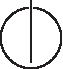
\includegraphics[height=20mm]{include/logos/faculty.pdf}
  }{}
\end{titlepage}


\frontmatter{}

\begin{titlepage}
  \centering

  \oTUM{38mm}

  \vspace{5mm}
  \begin{spacing}{1.55}
    {\huge\MakeUppercase{\getFaculty{}}}\\
  \end{spacing}

  \vspace{5mm}
  {\large\MakeUppercase{\getUniversity{}}}\\

  \vspace{20mm}
  {\Large \getDoctype{}}

  \vspace{15mm}
  {\huge\bfseries \getTitle{}}

  \vspace{10mm}
  {\huge\bfseries \getTitleGer{}}

  \vspace{10mm}
  \begin{tabular}{l l}
    Author:          & \getAuthor{}         \\
    Supervisor:      & \getSupervisor{}     \\
    Advisor:         & \getAdvisor{}        \\
    Submission Date: & \getSubmissionDate{} \\
    % \ifdraft{Version: & \today ~(Draft)\\}{}
  \end{tabular}

  \IfFileExists{include/logos/faculty.pdf}{%
    \vfill{}
    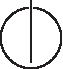
\includegraphics[height=20mm]{include/logos/faculty.pdf}
  }{}
\end{titlepage}
\cleardoublepage{}

\thispagestyle{empty}
\vspace*{0.8\textheight}
\noindent
I confirm that this \MakeLowercase{\getDoctype{}} is my own work and I have documented all sources and material used.

\vspace{15mm}
\noindent
\getSubmissionLocation{}, \today \hspace{50mm} \getAuthor{}

\cleardoublepage{}

% \phantomsection{}
\addcontentsline{toc}{chapter}{Acknowledgments}
\thispagestyle{empty}

\vspace*{20mm}

\begin{center}
{\usekomafont{section} Acknowledgments}
\end{center}

\vspace{10mm}

% Please DONT use all the titles in the Acks and also not the Makros
I would like to express my gratitude to my advisor \getAdvisor{} and my supervisor \getSupervisor{} for the opportunity to work on this interesting topic.

Furthermore, I would like to thank Max for the thesis template. 

Many people, especially my friends have made valuable suggestions on my thesis. Without your ideas and corrections, the thesis would not be as good as it is now. Thanks to my roommates for proofreading and providing ideas throughout the whole process of writing. Thanks to my apartment for letting me live in it. You get the idea.

This section is completely optional and you may also structure is as you like. Writing it in german is also fine.


\cleardoublepage{}

\chapter{Abstract}

We present a framework for students to bootstrap your final thesis. The primary goal of this template is to improve the quality of the thesis by avoiding typical mistakes. Our framework focuses on the basic thesis structure, which is mostly applicable, and helps you to immediately start writing. The first step is that the student writes down what he did so far, and performs some changes to this structure, yielding a thesis with notes and a rough plan how to write it up. The second step is to transform your notes into sentences, yielding a first draft. A template is the first step to the final thesis. In contrast to writing a thesis from scratch, our approach gives you a scaffold and helps you focusing on the important parts. We also show how to plot your data and describe your experiments. We present experimental results showing the perfect final thesis in the end.

As you might already have noticed, the abstract is the first, and sometimes only part the reader notices.
Thus it's crucial to summarize your work while motivating the reader here.
To help you with formulating we provide a basic structure to just fill the gaps.
Afterward, you can and should reformulate it to add your personal touch to it.

[...] present [...] for [...] to [...]. The primary goal of [...] is to improve [...] by avoiding [...] . Our framework focuses on [...], which is [...] , and is [...]. The first [...] , and performs [...], yielding [...]. The second [...] where [...], and yields [...]. [...] is the first [...]. In contrast [...], our approach [...]. We also show how [...]. We present experimental results showing [...].
 

\chapter{Kurzfassung}

In case you are not speaking german, you are free to drop the german abstract.

Dies ist der einzige Teil der Arbeit auf deutsch. 
Die Kurzfassung ist optional.
Sie erfüllt den gleichen Teil wie der englische Abstract, ist aber wahrscheinlich ein bisschen verständlicher, wenn ihr eure Arbeit daheim zeigt.
\microtypesetup{protrusion=false}
\tableofcontents{}
\listoffixmes{}
\microtypesetup{protrusion=true}
\mainmatter{}

\chapter{Introduction}\label{c:introduction}

During his speech "Null Reference: The Billion Dollar Mistake" in 2009, Tony Hoare, a renowned computer scientist, well known for the invention of Quick-sort, proposed the idea of how null pointers are the reason for at least a billion dollars in damages \cite{billiondollarmistake}. This quote could not be more important than at this time. In July 2024, Microsoft devices faced what has been described as the "most spectacular IT meltdown the world has ever seen" \cite{bloombergmeltdown}. This meltdown affected 8.5 million Microsoft Windows devices and severely impacted public institutions, including critical infrastructure like hospitals and airports \cite{bloomberg8milliondevices}. In the root cause analysis paper by Crowdstrike, the cybersecurity company that deployed the faulty code, it was revealed that inproper compile time validation and missing runtime array bounds checks were a big part of the error \cite{crowdstrikerca}.

The damage that can be done by a single ring 0 driver like Crowdstrike's Falcon software shows how critical it is to ensure memory safety. By using Rust, a memory-safe yet highly performant programming language with a restrictive compiler, we could drastically improve security and memory safety. We can witness Rust's influence on the systems development community since even the Linux kernel, which has been using C for almost 30 years without accepting any other languages like C++, now allows Rust code in its codebase \cite{linuxrustpull}.

However, it's also important to consider Rusts safety limits. While using Rust for a driver improves the overall safety of the process while not compensating on performance, direct memory and I/O operations have to be implemented in an unsafe way. A userspace driver using physical DMA addresses enables a device to practically have full access to the memory and potentially do detrimental I/O operations. Malicious firmware attacks are a rising threat.
To enforce safety at the device level, we need to make use of the IOMMU, a safe way of doing direct memory accesses. The IOMMU acts as a layer of isolation between devices and the CPU. By using virtual addresses, the IOMMU provides a bigger virtual address space and enforce memory access rights \cite{OLS2007}.

The primary goal of this thesis is to examine how the IOMMU impacts performance in the context of userspace I/O.
We demonstrate this by implementing IOMMU support on vroom, a NVMe driver written in Rust \cite{vroom}, and comparing it to using physical addresses. We use the Linux framework VFIO to implement the IOMMU functionality, which has the additional benefit of enabling the driver to run without root privileges. Additionally, we will be looking at IOMMUFD, a modern replacement for VFIO's IOMMU API.

\chapter{Background}

\section{vroom}
vroom currently uses hugepages and locks them using mlock to prevent the Kernel from swapping them out. 
This only enables the use of 2MiB hugepages, which can be disadvantageous for certain applications that would benefit from smaller page sizes.
A NVMe driver consists of submission and completion queues, implemented as ring buffers. 
The driver adds commands to the submission queue, which the NVMe controller reads and executes. 
The executed command gets placed on a corresponding completion queue.
For accessing the devices memory as well as the device accessing the host memory, it is necessary to either use the physical addresses and compromise on safety and use root privileges or use the IOMMU for virtualization, which can introduce performance overhead. 

\section{IOMMU}
The IOMMU works similarly to the MMU in the CPU, mapping physical addresses to virtual addresses.
The IOMMU does this by performing page table walks, through which a physical address is translated to a virtual address.
To improve performance on the IOMMU, an IOTLB is used to cache translations.

\section{IOTLB}
As page table walks are rather costly in performance, a cache on the IOMMU is used to store previously calculated addresses. This cache is called the Input/Output Translation Lookaside Buffer. The IOTLB possesses a limited capacity for entries. 

\section{VFIO}
VFIO is an IOMMU agnostic framework for exposing devices to userspace. 
This allows the driver to be safe and non-privileged in comparison to directly mapping the device memory to userspace. 

\section{IOMMUFD}
IOMMUFD is a user API for exposing DMA to userspace. 
It allows management of I/O address spaces (IOAS), enabling mapping/unmapping user space memory on the IOMMU.

\chapter{Related Work}

\section{SPDK}
\section{IOMMUFD}
\chapter{Implementation}

\section{Virtual Function I/O}
Virtual Function I/O (VFIO) is an IOMMU agnostic framework for exposing devices to userspace.
The VFIO driver binds to the PCI device and manages address translation through the IOMMU.
This allows the driver to be safe and non-privileged in comparison to directly mapping the device memory to userspace.
Using the VFIO works by using ioctl system calls.
While there is Rust's extensive \texttt{libc} library providing the system calls \texttt{ioctl} and \texttt{mmap} and their flags, the Linux \texttt{vfio.h} constants and structs need to either be defined manually or with a crate like bindgen, which automates bindings for C and C++ libraries \cite{cratebindgen}. To keep the binary and dependency list as small as possible we chose the manual implementation.


\subsection{Initialising the IOMMU}

To use the IOMMU for the driver, we first need to initialize the VFIO kernel module and bind the VFIO driver to the NVMe device.
As this binds the driver to a device, it has to be run with root privileges.
By changing the owner of the VFIO container to an unprivileged user, the driver can use the VFIO driver to interact with the device without root.
In \autoref{lst:vfioinit} the initialization script for the Vfio driver is shown.

\begin{lstlisting}[language=bash,caption={Initializing VFIO using bash}, label=lst:vfioinit, frame=single]
    #!/bin/bash
    modprobe vfio-pci
    nvme_vd="$(cat /sys/bus/pci/devices/$nvme/vendor) $(cat /sys/bus/pci/devices/$nvme/device)"
    echo $nvme > /sys/bus/pci/devices/$nvme/driver/unbind
    echo $nvme_vd > /sys/bus/pci/drivers/vfio-pci/new_id
    chown $user:$group /dev/vfio/*     
\end{lstlisting}

\begin{enumerate}
    \item Add VFIO kernel module using \texttt{modprobe}
    \item Unbind kernel driver from NVMe
    \item Use vendor and device id to bind VFIO to the device
    \item Set VFIO group permissions to user/group using \texttt{chown}
\end{enumerate}

\subsection{Initialising the NVMe device}
Using the Vfio, the initialization process of the NVMe SSD works as followed.

\begin{enumerate}
    \item Map the NVMe device memory into host memory using VFIO resource info.
    \item Allocate Admin SQ, CQ and I/O SQ, CQ
    \item Create a mapping on the IOMMU using VFIO
    \item Configure the NVMe device
    \item Pass I/O Queue addresses to NVMe device using admin queues
\end{enumerate}

\subsection{Enabling DMA}
To enable DMA we need to set a bit in the PCIe device registers.

\subsection{Mapping DMA}
In order to provide a section of memory on which the device can perform DMA operations, the user needs to allocate some memory in the processes address space. This can be achieved by using the Linux syscall \texttt{mmap}.
Using \texttt{mmap}'s flags we can also define the page size used.
The \texttt{MAP\_HUGETLB} flag is used in conjunction with the \texttt{MAP\_HUGE\_2MB} and \texttt{MAP\_HUGE\_1GB} flags for 2MiB and 1 GiB pages respectively.
By default \texttt{mmap} uses the default page size of 4KiB.
The main IOMMU work is done by then creating the map struct \texttt{vfio\_iommu\_type1\_dma\_map}. We set the DMA mapping to read and write, and provide the same IOVA as the Virtual address. By then passing it to an ioctl call with the according VFIO operation \texttt{VFIO\_IOMMU\_MAP\_DMA} we can create a mapping in the page tables of the IOMMU. This way we can give the IOVA to the NVMe controller, which it will use to access the memory through the address translation of the IOMMU.
On \autoref{fig:vroom-graph} an I/O operation timeline graph can be seen.

\begin{figure}
    \centering
    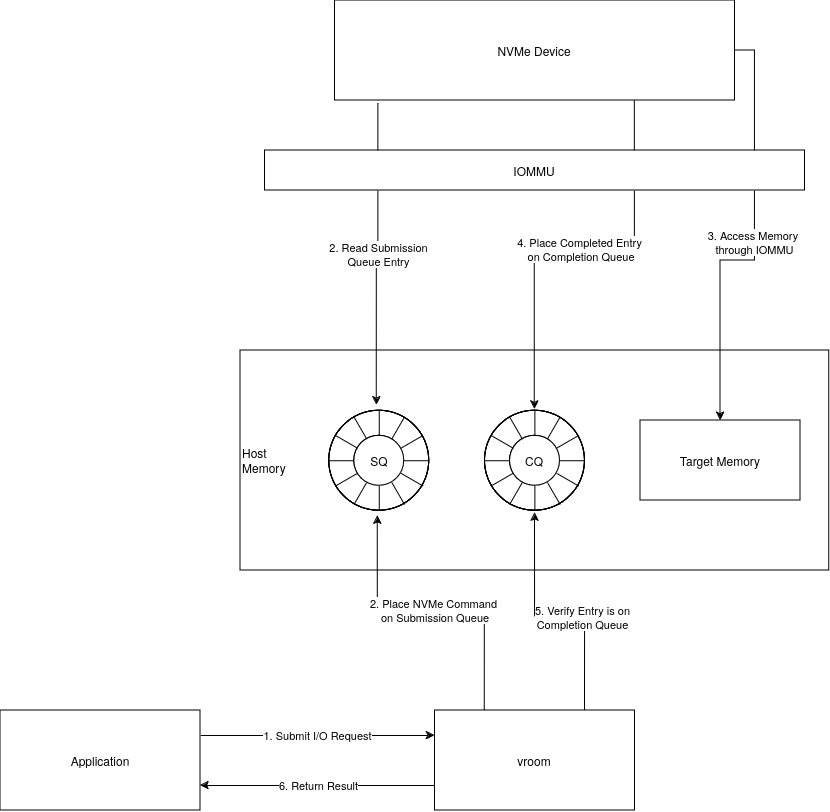
\includegraphics[width=\textwidth]{figures/vroomgraphlight.png}
    \caption{I/O operation vroom}
    \label{fig:vroom-graph}
\end{figure}

\subsection{Unmapping DMA}
Unmapping DMA happens when the process exits, yet for performance and application reasons there is the unmap\_dma function which can be used to unmap a DMA. It is necessary to increase the allocated size to a multiple of the page size as otherwise the munmap operation will result in a failure.

\subsection{Regions}
Using regions, we can directly mmap device memory into host memory for easy access to the NVMe controller.
VFIO provides structs for using mmap to directly map the NVMe device into memory. Using \texttt{VFIO\_DEVICE\_GET\_REGION\_INFO} we can attain the length and the offset needed for mmap.

\subsection{Groups and Containers}
VFIO uses group to distinguish between groups of devices which can be isolated from the host system. In the ideal case, every device would only be part of one group in order to increase security by providing single-device isolation. Groups are the smallest unit size on a system to ensure secure user access.
To further reduce overhead from the IOMMU Containers are used in VFIO, which can hold multiple groups. These containers can be used to ease translation and reduce TLB page faults.
In our implementation we use one group and container each for our NVMe device.

\section{IOMMUFD}
The IOMMU File Descriptor user API (IOMMUFD) offers a way of controlling the IOMMU subsystem using file descriptors in user-space \cite{iommufdkerneldocs}.
It allows management of I/O address spaces (IOAS), enabling mapping user space memory on the IOMMU.
IOMMUFD has only been recently added to the Linux Kernel in December of 2022. E.g. Debian 12 does not include it, Fedora 40 does, but it is not enabled in the kernel configuration. Considering that it is not widely available or enabled on many distributions, our driver offers both options of using the IOMMU. The performance tests are done using the 'legacy' VFIO-only way, but it can be assumed that the framework/user api does not have a noteworthy performance impact.
The device file descriptor, which was previously attained with \texttt{VFIO\_GROUP\_GET\_DEVICE\_FD} can now be gotten through opening the character device /dev/vfio/devices/vfioX.
By using this character device pointer we can claim the ownership over the VFIO device. That way VFIO does not rely on group/container/iommu drivers.

\subsection{IOAS}

\chapter{Evaluation}
In this chapter, we analyze the performance impact of the IOMMU, directly comparing it to the physical address approach. To compare both approaches fairly, we allocate and map the memory upfront. The focus lies on the IOMMU itself and how it performs. All performance tests use legacy VFIO instead of IOMMUFD as it currently remains the widely supported way of using the IOMMU.

\section{Setup}
We use two systems to benchmark the driver's performance.
Both systems run Ubuntu 23.10 with Linux kernel version 6.5.0-42 and are NUMA systems with two nodes each. We stick to NUMA locality, ensuring that the tested processes access memory from their nearest available memory node to improve performance.

\begin{table}[H]
  \centering
  \begin{tabular}{lllrll}
    \textbf{CPU}                          & \textbf{Memory}                         & \textbf{NVMe}                         & \textbf{Capacity}                       & \textbf{Count}   \\
    \toprule

    \multirow{2}{*}{Intel Xeon E5-2660v2} & \multirow{2}{*}{\qty{251}{\gibi\byte}}  & \multirow{2}{*}{Samsung Evo 970 Plus} & \multirow{2}{*}{\qty{1}{\tera\byte}}    &
    \multirow{2}{*}{1}                                                                                                                                                                   \\
                                          &                                         &                                       &                                         &                & \\ \hline

    \multirow{2}{*}{AMD EPYC 7713}        & \multirow{2}{*}{\qty{1007}{\gibi\byte}} & \multirow{2}{*}{Samsung PM9A3}        & \multirow{2}{*}{\qty{1.92}{\tera\byte}} &
    \multirow{2}{*}{8}                                                                                                                                                                   \\
                                          &                                         &                                       &                                         &                & \\
    \bottomrule
  \end{tabular}

  \caption{Specifications of systems used in performance testing}
  \label{tab:servers}
\end{table}

\begin{table}[H]
  \centering
  \begin{tabular}{llrrrr}
    \multirow{2}{*}{\textbf{CPU}} & \multirow{2}{*}{\textbf{Clock}} & \multirow{2}{*}{\textbf{Cores}} & \multirow{2}{*}{\textbf{Virtualization}} & \multirow{2}{*}{\textbf{Year}}
    \\
                                  &                                 &                                 &                                          &                                \\
    \toprule

    Intel Xeon E5-2660v2          & \qty{2.2}{\giga\Hz}             & 10                              & VT-d                                     & 2012                           \\
    AMD EPYC 7713                 & \qty{2.0}{\giga\Hz}             & 64                              & AMD-V                                    & 2021                           \\

    \bottomrule
  \end{tabular}

  \caption{CPUs of the systems}
  \label{tab:cpus}
\end{table}

\begin{table}[H]
  \centering
  \begin{tabular}{lrrll}
    \multirow{2}{*}{\textbf{NVMe}} & \textbf{Maximum}     & \textbf{Maximum}    & \multirow{2}{*}{\textbf{Turbowrite}} & \multirow{2}{*}{\textbf{Usage}} \\
                                   & \textbf{Queue Count} & \textbf{Queue Size} &                                      &                                 \\
    \toprule

    Samsung Evo 970 Plus           & 128                  & 16384               & Yes                                  & Consumer                        \\
    Samsung PM9A3                  & 128                  & 16384               & No                                   & Enterprise                      \\

    \bottomrule
  \end{tabular}

  \caption{NVMe(s) of the systems}
  \label{tab:nvmes}
\end{table}

Despite the NVMe specification's maximum capability of 65536 I/O queues, our SSDs support a more reasonable amount of 128 I/O queues, which seems to be typical for modern SSDs.
Turbowrite is a Samsung technology that drastically speeds up write latencies in the so-called "Turbowrite" buffer with the size of \qty{42}{\giga\byte} of the NVMe, as shown in \cite{vroom}. All NVMe SSDs used were formatted to 512-byte blocks.

We use one thread per 1 I/O queue in our multithreaded tests.
All writes are performed on an empty SSD to avoid overhead through garbage collection on the NVMe. As the NVMe can optimize reads on an empty SSD, all reads will be performed on a full SSD. We exclusively use random writes/reads for the tests, as the NVMe can drastically optimize sequential requests, which can lead to altered results.
Unless stated otherwise, we configure the submission and completion queue length to the maximum amount supported by the NVMes.
Additionally, all standard tests are run with the \texttt{iommu.strict=1} kernel parameter. When this parameter is set, the IOMMU invalidates the complete IOTLB when an unmapping occurs. As we unmap IOVAs in between tests, this ensures that the IOTLB is flushed before each test.

\section{Results}
For the following performance tests, we will compare the latencies and throughput of vroom without the IOMMU and with the IOMMU, both utilizing \qty{2}{\mebi\byte} pages. All latency and throughput tests are run with a \qty{1}{\gibi\byte} buffer in memory. For \qty{2}{\mebi\byte} pages, this equates to 512 pages being accessed. We use a unit size of \qty{4}{\kibi\byte}, i.e., each I/O operation reads/writes \qty{4}{\kibi\byte} to the the NVMe.

\subsection{Latencies}
All latency performance measurements are done singlethreaded with queue depth 1 over a timespan of 60 seconds.

\begin{figure}[H]
  \centering
  \subcaptionbox {Random read} {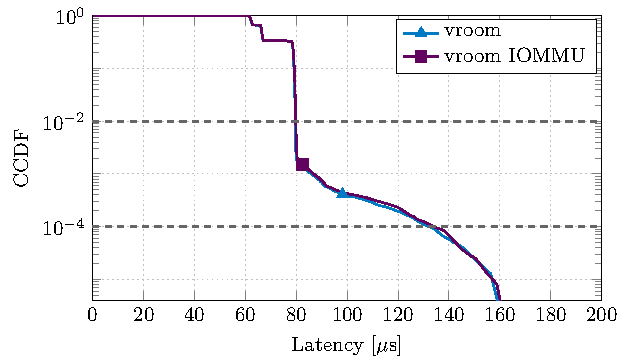
\includegraphics[width=.70\textwidth]{figures/lats_ccdf_2MiB_qd1t1_read} \label{fig:ccdf-read}}
  \subcaptionbox {Random write} {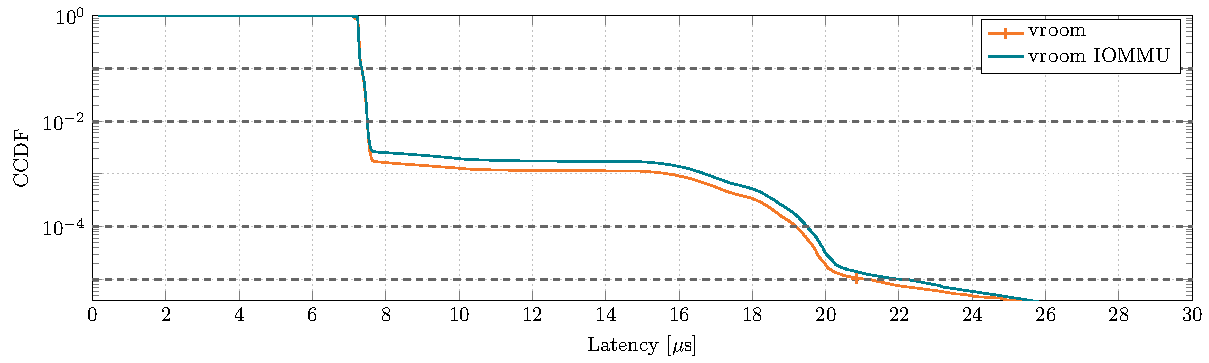
\includegraphics[width=.70\textwidth]{figures/lats_ccdf_2MiB_qd1t1} \label{fig:ccdf-write}}
  \caption{Tail latencies (60s) on Intel System}
  \label{fig:ccdf}
\end{figure}

\begin{figure}[H]
  \centering
  \subcaptionbox {Random read} {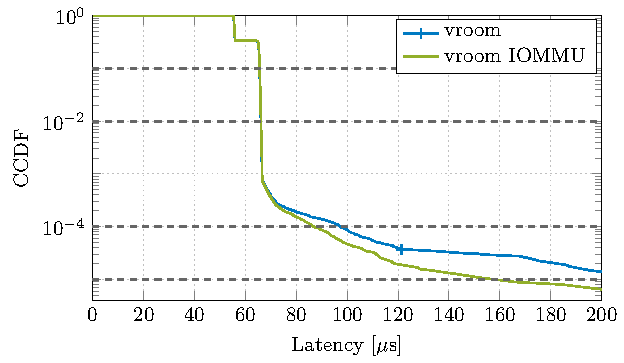
\includegraphics[width=.70\textwidth]{figures/lats_ccdf_2MiB_qd1t1_read_epyc} \label{fig:ccdf-read-epyc}}
  \subcaptionbox {Random write} {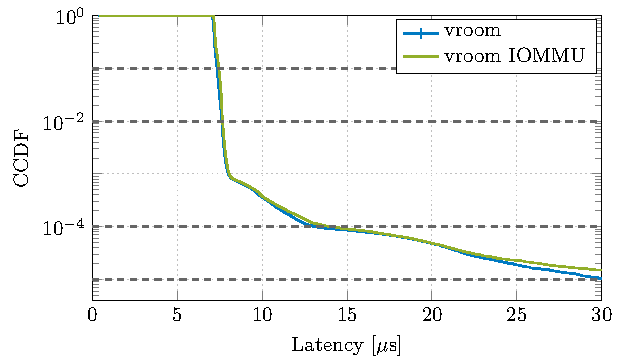
\includegraphics[width=.70\textwidth]{figures/lats_ccdf_2MiB_qd1t1_epyc} \label{fig:ccdf-write-epyc}}
  \caption{Tail latencies (60s) on AMD System}
  \label{fig:ccdf-epyc}
\end{figure}

\autoref{fig:ccdf} and \autoref{fig:ccdf-epyc} show that the latency distribution is the same with IOMMU as without. The lines are mostly overlapping. This shows that there are no significant latency spikes that occur due to the IOMMU.

\subsection{Throughput}
To test the overall throughput we perform random reads/writes over 60 seconds once with singlethreaded I/O and queue depth 1 and once with queue depth 32 and 4 threads. As seen on \autoref{fig:throughput-bar}, the IOMMU has no noticeable performance impact. Even with the higher queue depth and thread count, the performance is identical.

\begin{figure}[H]
  \centering
  \subcaptionbox {Queue depth 1 and 1 thread} {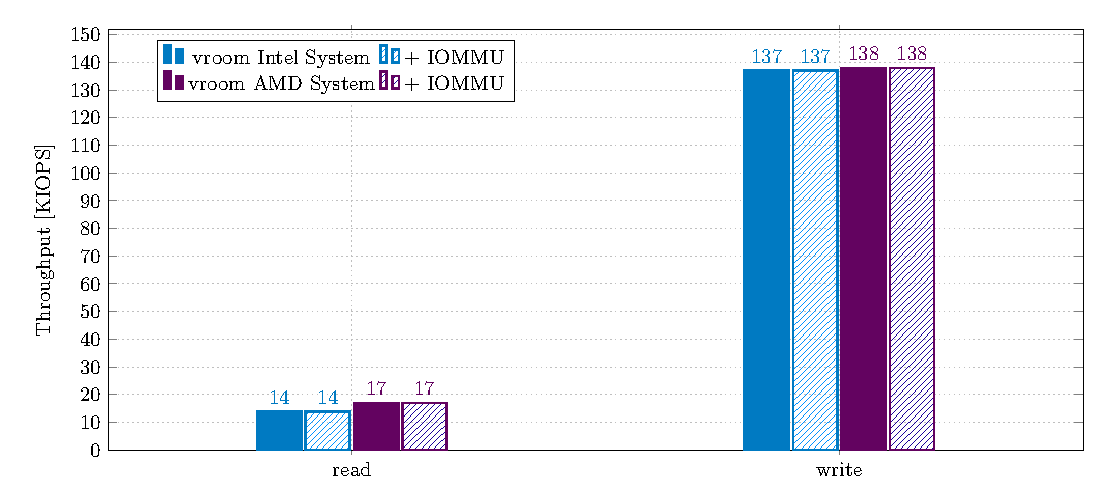
\includegraphics[width=.9\textwidth]{figures/throughput_bar_qd1t1} \label{fig:throughput-qd1t1}}
  \subcaptionbox {Queue depth 32 and 4 threads} {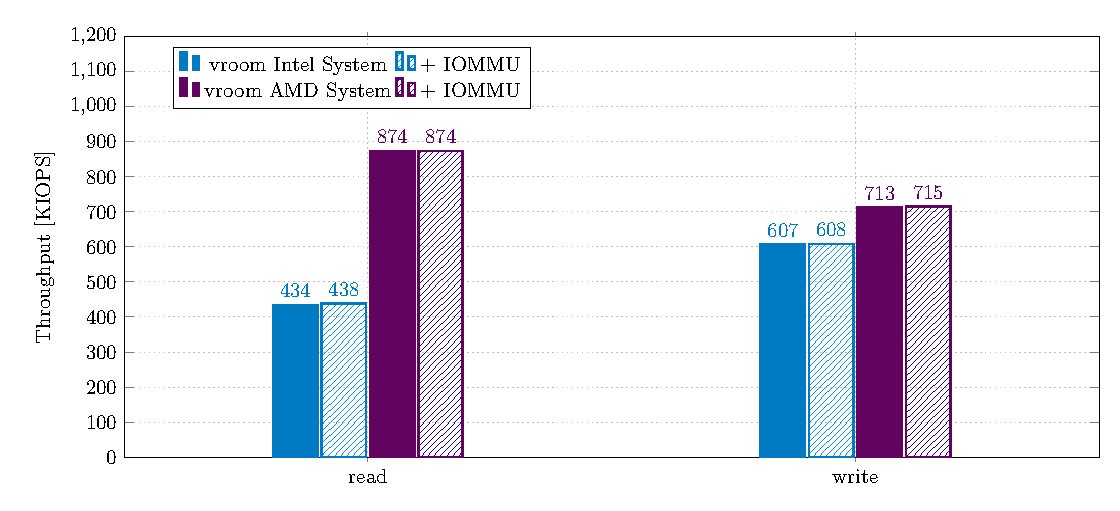
\includegraphics[width=.9\textwidth]{figures/throughput_bar_qd32t4} \label{fig:throughput-qd32t4}}
  \caption{Throughput of singlethreaded and multithreaded I/O over 60s}
  \label{fig:throughput-bar}
\end{figure}

We also take a look at throughput performance with larger queue depths. The performance is mostly the same, but a slight performance difference is noticeable on the AMD system, where the maximum throughput of vroom with IOMMU is around 3\% higher than without the IOMMU.

\begin{figure}[H]
  \centering
  \subcaptionbox {Intel System} {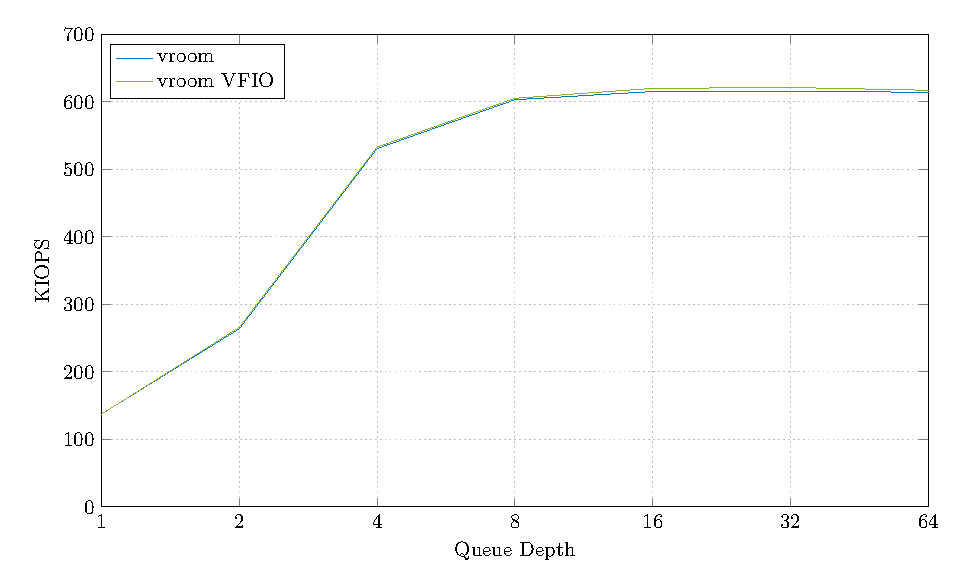
\includegraphics[width=.8\textwidth]{figures/qdnt1_2MiB} \label{fig:qdnt1-2MiB-intel}}
  \subcaptionbox {AMD System} {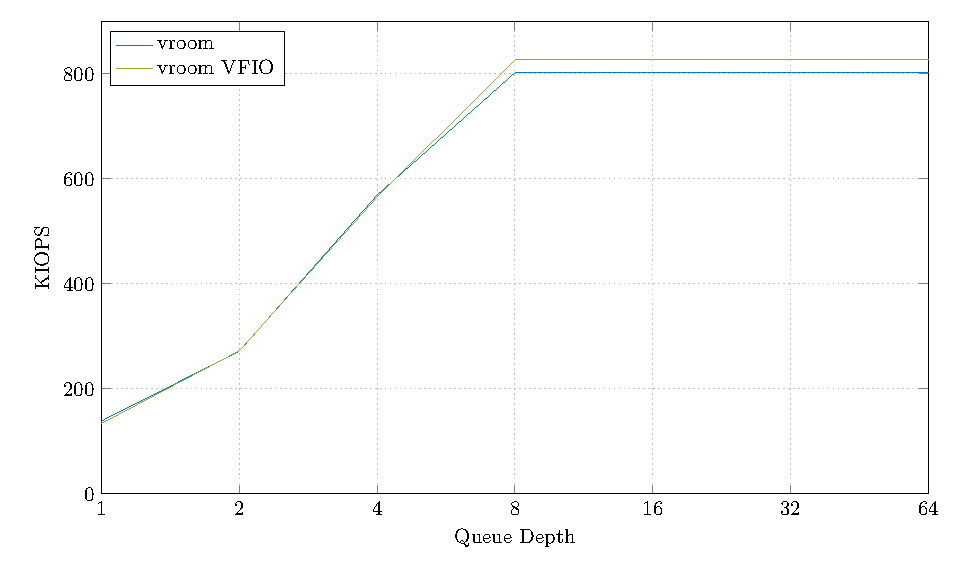
\includegraphics[width=.8\textwidth]{figures/qdnt1_2MiB_epyc} \label{fig:qdnt1-2MiB-epyc}}
  \caption{Random write throughput with increasing Queue Depth over 60s}
  \label{fig:qdnt1-2MiB}
\end{figure}

\paragraph{Using multiple SSDs} We further push the throughput by using 8 NVMes with high queue depth and thread counts in parallel in \autoref{fig:throughput-bar-8n}. Again, no significant performance impact occurs. Each NVMe has a slightly higher throughput than when tested alone.

\begin{figure}[H]
  \centering
  \subcaptionbox {Queue depth 1 and 1 thread\label{fig:throughput-qd1t1-8n}} {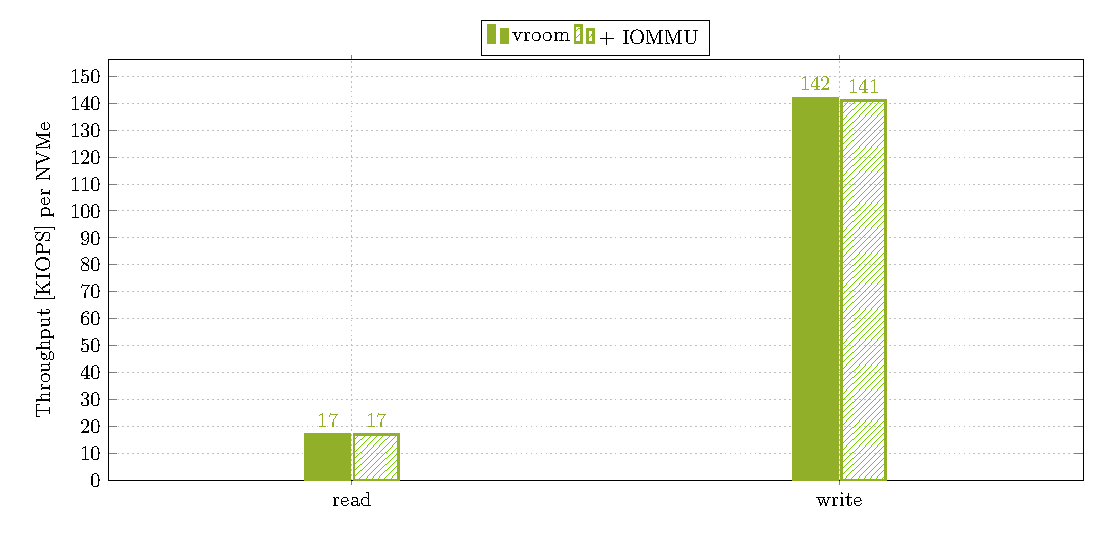
\includegraphics[width=.7\textwidth]{figures/throughput_bar_qd1t1_8nvmes} }
  \subcaptionbox {Queue depth 32 and 4 threads\label{fig:throughput-qd32t4-8n}} {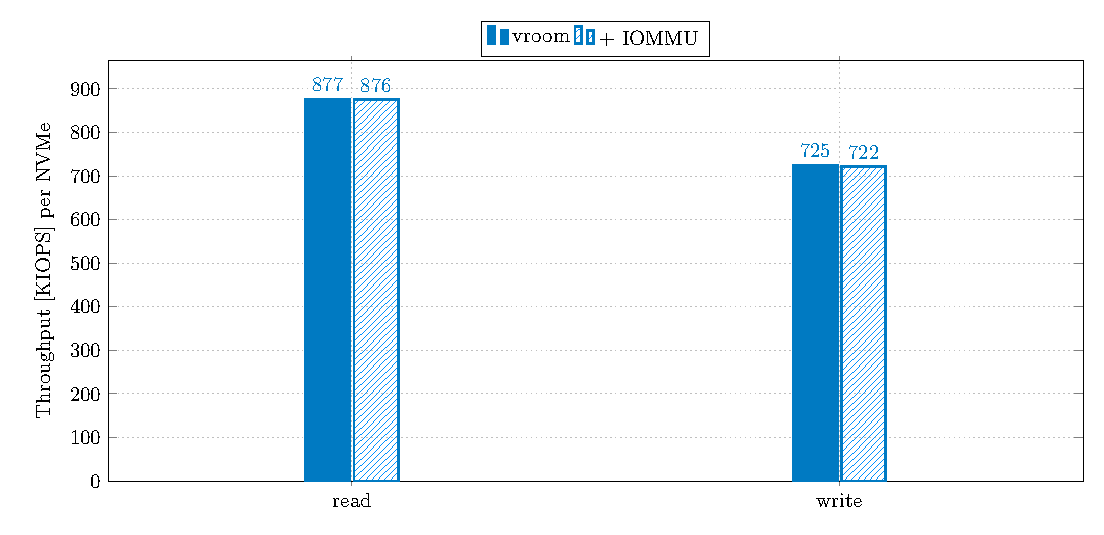
\includegraphics[width=.7\textwidth]{figures/throughput_bar_qd32t4_8nvmes} }
  \subcaptionbox {Queue depth 128 and 16 threads\label{fig:throughput-qd128t16-8n}} {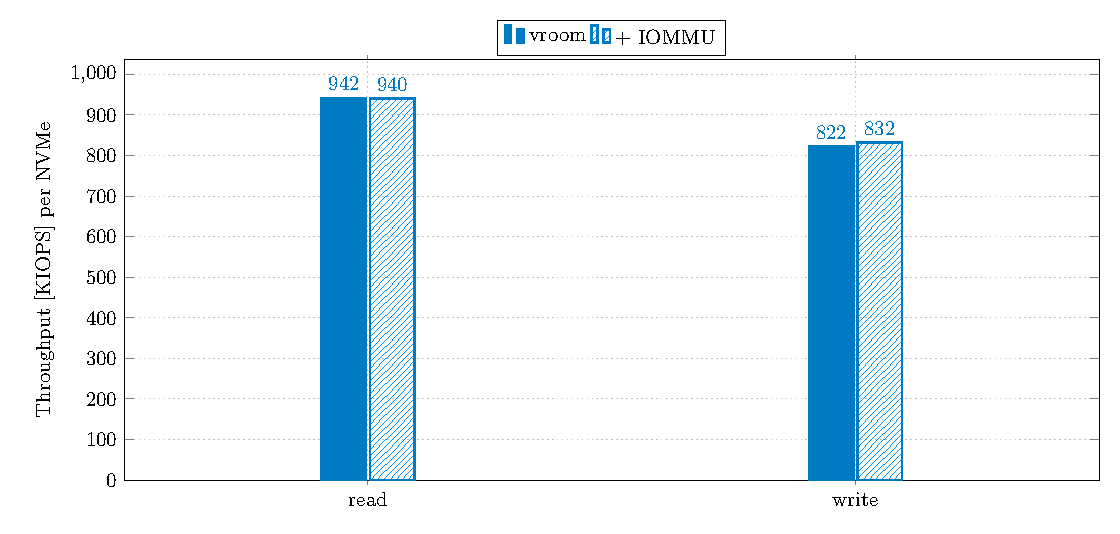
\includegraphics[width=.7\textwidth]{figures/throughput_bar_qd128t16_8nvmes} }
  \caption{Throughput over 60s on 8 NVMe SSDs on the AMD system}
  \label{fig:throughput-bar-8n}
\end{figure}

\section{Impact of \qty{4}{\kibi\byte} pages}
\subsection{Throughput}
As Linux, as well as our IOMMUs, support \qty{4}{\kibi\byte}, \qty{2}{\mebi\byte} and \qty{1}{\gibi\byte} page sizes, we will test and analyze how it affects the latencies and overall performance. A performance impact should be noticeable, especially using \qty{4}{\kibi\byte} pages. As we use a typical unit size of \qty{4}{\kibi\byte}, using \qty{4}{\kibi\byte} pages should result in TLB-thrashing, i.e., every I/O operation resulting in a page walk. To test this hypothesis, we focus on the Intel system and only write to the Turbowrite buffer of the Samsung Evo 970 Plus to reach the maximum performance and lowest latencies. We test this using an increasing number of threads in \autoref{fig:qd1tn-4kib} and an increasing queue depth in \autoref{fig:qdnt1-4kib}.

\begin{figure}[H]
  \centering
  \subcaptionbox {1 \qty{4}{\kibi\byte} buffer per thread} {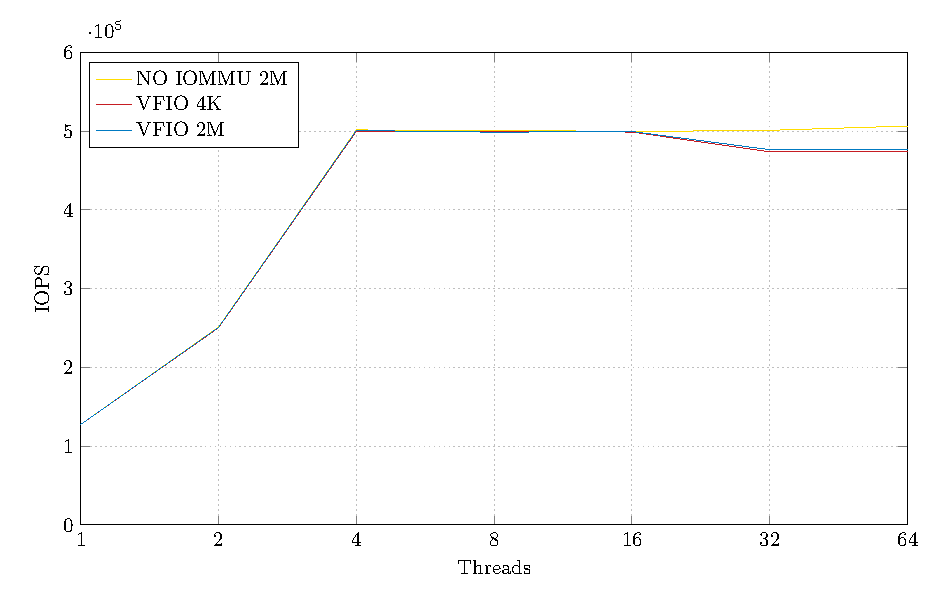
\includegraphics[width=0.6\textwidth]{figures/qd1tn_1page}}
  \subcaptionbox {1 \qty{2}{\mebi\byte} buffer per thread} {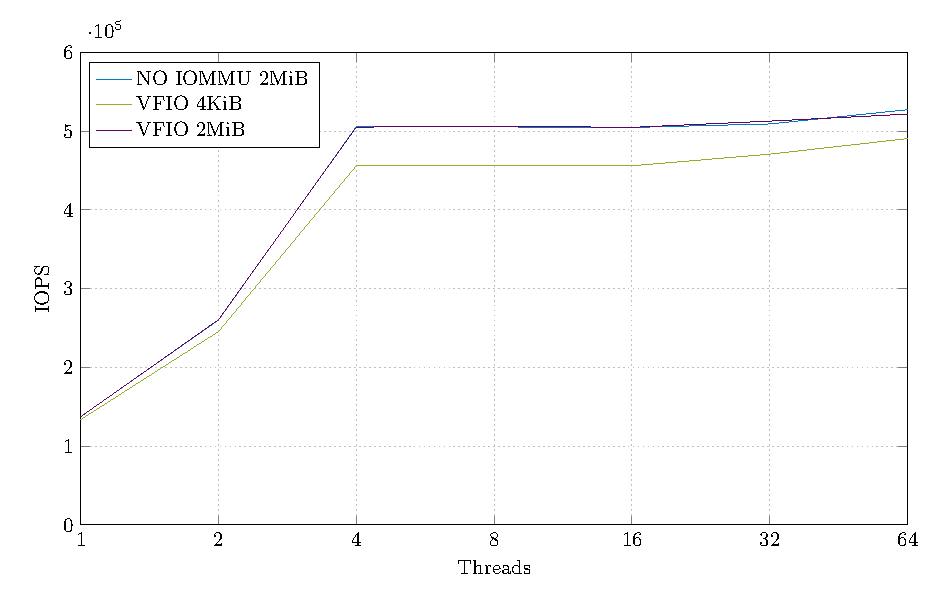
\includegraphics[width=0.6\textwidth]{figures/qd1tn_512page}}
  \caption{Random write throughput over 20s with increasing thread count and queue depth 1 on the Intel system}
  \label{fig:qd1tn-4kib}
\end{figure}

In \autoref{fig:qd1tn-4kib}, when comparing the performance of vroom without the IOMMU against vroom with IOMMU using \qty{4}{\kibi\byte} and \qty{2}{\mebi\byte} pages on a 2MiB buffer, a performance difference of around 10\% between \qty{4}{\kibi\byte} pages and \qty{2}{\mebi\byte} pages can be observed. This stems from the aforementioned IOTLB-thrashing. Noticeable is that no performance impact can be seen when using a 4KiB buffer, as all pages can fit into the IOTLB. The lines of both implementations using \qty{2}{\mebi\byte} pages overlap with both buffer sizes.

\begin{figure}[H]
  \centering
  \subcaptionbox {1 \qty{4}{\kibi\byte} buffer per thread} {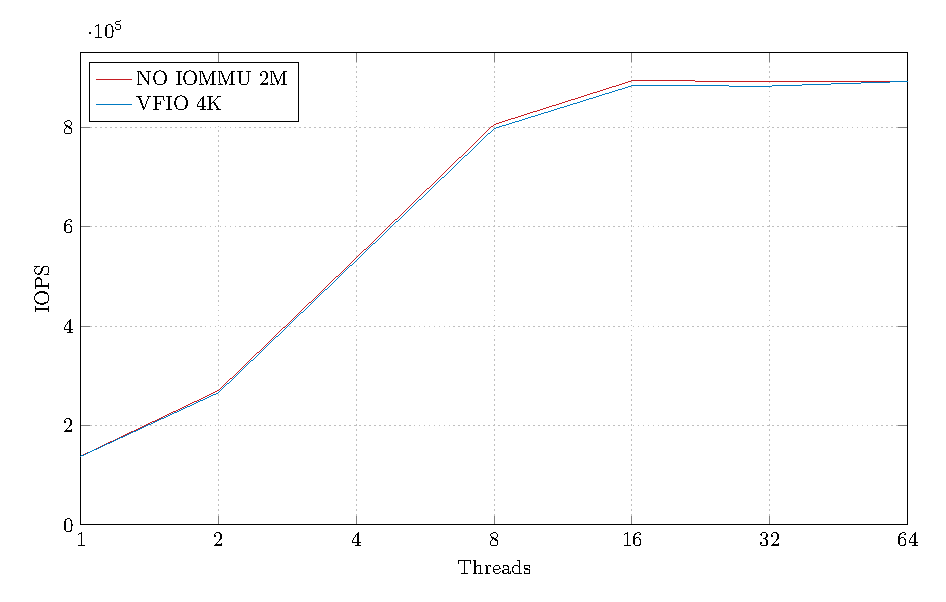
\includegraphics[width=0.6\textwidth]{figures/qdnt1_1page}}
  \subcaptionbox {1 \qty{2}{\mebi\byte} buffer per thread} {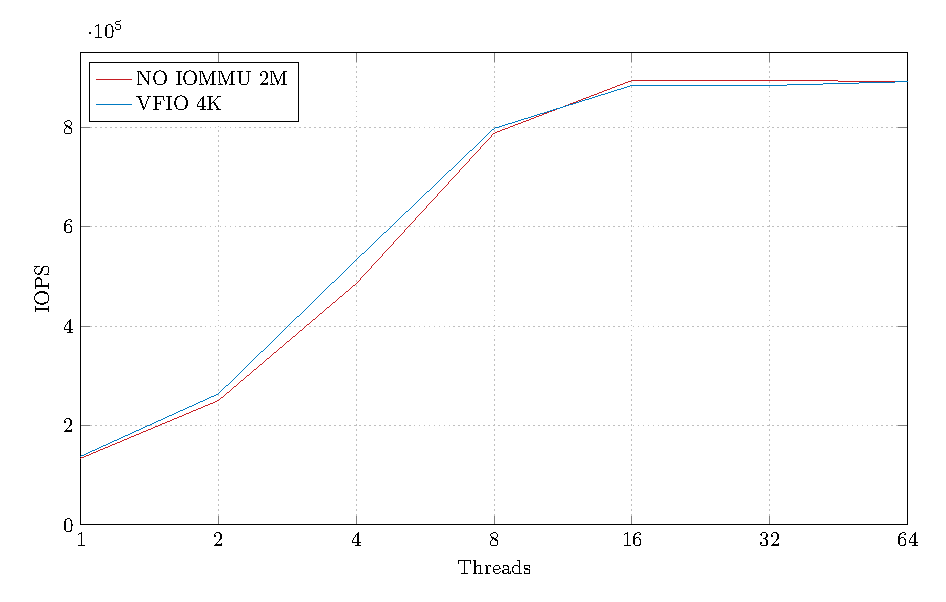
\includegraphics[width=0.6\textwidth]{figures/qdnt1_512page}}
  \caption{Singlethreaded random write throughput over 20s with increasing queue depth on the Intel system}
  \label{fig:qdnt1-4kib}
\end{figure}

In \autoref{fig:qdnt1-4kib}, a 10\% performance decrease can be seen at queue depth 4. This difference grows smaller as we further increase the queue depth, though. At 16 or more queue depth the throughput caps at around 890KIOPS, and no more substantial difference between the implementations can be measured. As we have seen a constant decrease of 10\% in performance when testing multiple threads in \autoref{fig:qd1tn-4kib}, we suspect that the PCIe bus is the bottleneck and limiting the performance.

\paragraph{PCIe limitations}
The Intel System SSD is mounted on a PCIe 3.0 4x width bus with a maximum payload of 256 bytes. This PCI bus has a maximum throughput of 3.938 GB/s. Using the SSD to its full capability, i.e. using random writes with high queue depths in the Turbowrite buffer, can result in the bus being the bottleneck. With the highest throughput measured being 890K IOPS with one I/O operation containing 4096 bytes of data, we achieve 3.64 GB/s. Including the headers for each TLP and submission- and completion queue entries, we come to a result of 3.908 GB/s. This roughly equates the PCIe bus limit and leads us to conclude, that the missing overhead of using \qty{4}{\kibi\byte} pages on high queue depths stems from this bottleneck.

\subsection{Determining IOTLB size}
As the size of the IOTLB is not stated in hardware and VT-d or AMD-V specifications, we use a latency test to analyze the behaviour of the IOMMU.
In order to isolate the effect of the IOMMU we track the latencies of the fastest operation the NVMe can perform. The lowest latency is achieved by carrying out a random write using the smallest block size of \qty{512}{\byte}.

If we then write from a single block from each page to the NVMe, repeat it 65536 times on an increasing page count that are a power of two, we can figure out where a latency spike occurs. The page count right before the latency spike should equal the IOTLB entry count. We configure the queues, buffer and prp-list to each take up one page, resulting in a maximum of 6 pages in the IOTLB before the actual workload.
The test is performed with VFIO with \qty{4}{\kibi\byte}, \qty{2}{\mebi\byte} and \qty{1}{\gibi\byte} pages and without the IOMMU with \qty{2}{\mebi\byte} pages as reference. As we have limited available memory, the \qty{1}{\gibi\byte} pages could only be tested to 112 pages on the Intel system and 128 on the AMD system.

\begin{figure}[H]
  \centering
  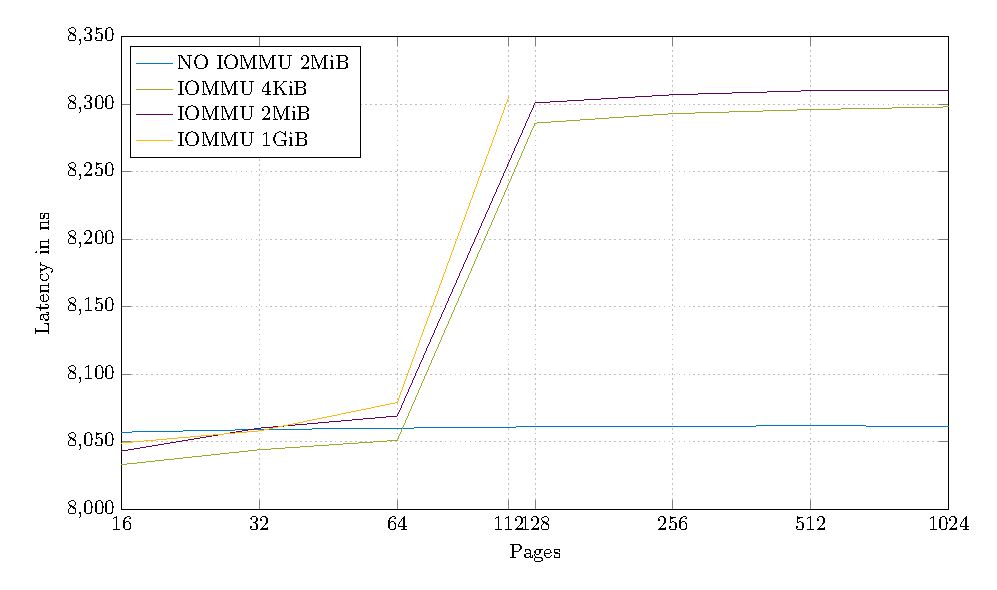
\includegraphics[width=\textwidth]{figures/psmeds}
  \caption{Latencies of random writes on an emptied SSD with increasing pages in memory on the Intel system}
  \label{fig:med-ps}
\end{figure}

\paragraph{Results of Intel Xeon E5-2660v2}
In the resulting graph \autoref{fig:med-ps} we can observe a performance spike of around 250 nanoseconds for each write between 64 and 128 allocated pages. In the case of \qty{4}{\kibi\byte} pages, this is a memory size of only 512 KiB. Using this information, we can assume that the IOTLB has the same size for each pagesize, as well as it \textbf{being 64 entries of size}. This matches the page size Stefan Huber and Rolf Neugebauer found \cite{iommuhuber}\cite{pcieperfnegebauer}.

\begin{figure}[H]
  \centering
  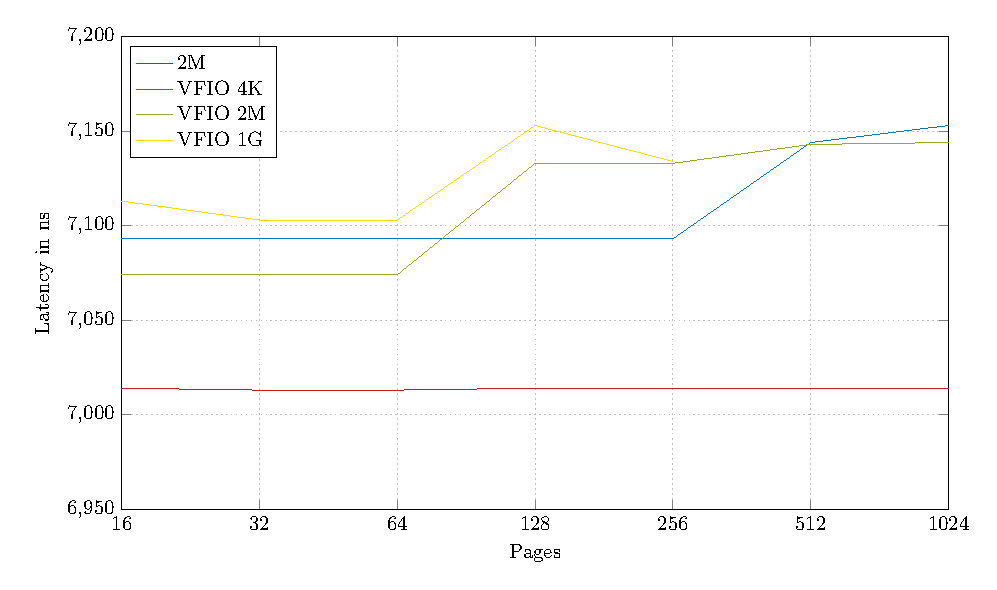
\includegraphics[width=\textwidth]{figures/psmedsepyc}
  \caption{Latencies of random writes on an emptied SSD with increasing pages in memory on the AMD system}
  \label{fig:med-psepyc}
\end{figure}

\paragraph{Results of AMD EPYC 7713}
On the AMD IOMMU, we can see three performance spikes. Each occurs between 32-64 pages for \qty{1}{\gibi\byte} pages, 64-128 pages for \qty{2}{\mebi\byte}, and 256-512 for \qty{4}{\kibi\byte} pages.
We can therefore assume that the IOTLB size depends on the pagesize unlike on the Intel CPU. This leads us to suspect an \textbf{IOTLB size of 32 for \qty{1}{\gibi\byte} pages, 64 for \qty{2}{\mebi\byte} pages and 256 for \qty{4}{\kibi\byte} pages}. The latencies only decrease by about \qty{60}{ns}, which is a about four times less than page walks on the Intel system.
\chapter{Conclusion}
In this thesis, we improved vroom's safety by implementing IOMMU support, by using the Linux framework VFIO.
We figured out the IOTLB size of two IOMMU models, which, when exceeded, can introduce address translation overhead for \qty{4}{\kibi\byte} pages.
When not exceeding the IOTLB, or using hugepages, the IOMMU performs extremely well, and practically no overhead can be seen.
The advantages of using the IOMMU, such as access rights and bigger address spaces, as well as the ability to run the driver without root privileges with VFIO, make it the preferred method of addressing memory.
Considering that IOMMU technology has seen a rise in popularity in the use of hardware passthrough for virtualization, it is likely that in the future, the IOMMU performance and the IOTLB size will increase, further closing any existing gap. The ability to improve security drastically and increase address space while not compromising on performance is the reason the MMU succeeded, and it is likely that the IOMMU will as well.

\paragraph{Rust in driver development}
The viability of using Rust to develop drivers has been shown often, and it has proved that a modern, memory-safe language like Rust can compete with C in systems development. Using Rust provides more safety and a modern ecosystem, a package manager, and zero-cost abstractions. This makes Rust an excellent choice for driver development.

\paragraph{Future Work}
Future Work on the driver could include expanding the NVMe capabilities. Currently, the driver is fixed to one namespace. Furthermore, the driver does not support a block device layer or file system. Including sysfs support could also be a next step.
Also, it could be investigated if and how many threads could operate on one I/O queue to further push the throughput. Finally, a performance investigation into IOMMUFD could be conducted, as we only tested the legacy VFIO model.

%\appendix{}
%\chapter{Implementation}\label{c:code}

%\begin{table}[htpb]
%    \centering
%    \begin{tabular}{r|l}
%        \textbf{\#} & \textbf{Category} \\
%        \hline
%\textbf{1} & Restaurants \\
%\textbf{2} & Food \\
%\textbf{3} & Nightlife \\
%\textbf{4} & Shopping \\
%\textbf{5} & Bars \\
%\textbf{6} & German \\
%\textbf{7} & Event Planning \& Services \\
%\textbf{8} & Cafes \\
%\textbf{9} & Coffee \& Tea \\
%\textbf{10} & Italian \\
%\textbf{11} & Hotels \& Travel \\
%\textbf{12} & Swabian \\
%\textbf{13} & Hotels \\
%\textbf{14} & Arts \& Entertainment \\
%\textbf{15} & Active Life \\
%\textbf{16} & Fashion \\
%\textbf{17} & Pizza \\
%\textbf{18} & Specialty Food \\
%\textbf{19} & Wine Bars \\
%\textbf{20} & International \\
%\textbf{21} & Fast Food \\
%\textbf{22} & Beer Garden \\
%\textbf{23} & Grocery \\
%\textbf{24} & Caterers \\
%\textbf{25} & Bakeries \\
%\textbf{26} & Pubs \\
%\textbf{27} & Cocktail Bars \\
%\textbf{28} & Burgers \\
%\textbf{29} & Music \& Video \\
%\textbf{30} & Books \\
%\textbf{31} & Mags \\
%\textbf{32} & Mediterranean \\
%\textbf{33} & Bistros \\
%\textbf{34} & Delicatessen \\
%\textbf{35} & Public Services \& Government \\
%\textbf{36} & Greek \\
%\textbf{37} & Lounges \\
%\textbf{38} & Breakfast \& Brunch \\
%\textbf{39} & Dance Clubs \\
%\textbf{40} & Beer \\
%\textbf{41} & Wine \& Spirits \\
%\textbf{42} & Music Venues \\
%\textbf{43} & Steakhouses \\
%\textbf{44} & Vegetarian \\
%\textbf{45} & French \\
%\textbf{46} & Venues \& Event Spaces \\
%\textbf{47} & Landmarks \& Historical Buildings \\
%\textbf{48} & Seafood \\
%\textbf{49} & Sports Clubs \\
%\textbf{50} & Party \& Event Planning \\
%\textbf{51} & Salad \\
%        \end{tabular}
%    \caption[Top 10 Categories in Stuttgart]{Top 10 Categories in Stuttgart}
%    \label{t:data:cities}
%\end{table}

\microtypesetup{protrusion=false}

\listoffigures{}
\listoftables{}
\lstlistoflistings{}

\microtypesetup{protrusion=true}

% Bibliographie Test
\printbibliography{}

\end{document}
